% =========================================================================== %

\begin{frame}[t,plain]
\titlepage
\end{frame}

% =========================================================================== %

\begin{frame}{About Me}
%
\begin{columns}
\column{.5\linewidth}
\begin{itemize}
\item Former Student of UR
	\begin{itemize}
	\item 2015-2021: Physics
	\item 2020-2022: Computational Science
	\item Have been involved in UR IT courses since 2018
	\end{itemize}
\item Now: Software Development Engineer
\item Hobby enthusiast since childhood
	\begin{itemize}
	\item First programming language (BASIC) when I was 9 years old
	\item So almost 25 years of semi-professional busying myself with computers
	\item I like sharing nerdy stuff in spite of my limited time
	\end{itemize}
\end{itemize}
%
\column{.5\linewidth}
\begin{itemize}
\item Human Languages
	\begin{itemize}
	\item German
	\item English
	\item French
	\end{itemize}
\item Computer Languages
	\begin{itemize}
	\item Python
	\item C, C++
	\item Java, Groovy
	\item BASIC (VisualBASIC, freeBASIC, QBASIC)
	\item \LaTeX
	\item (some Assembly, Bash Shell Scripting, Julia; even less HTML, CSS, PowerShell, MS-DOS Batch, MySQL, Maple, Matlab)
	\end{itemize}
\end{itemize}
\end{columns}
%
\end{frame}

% =========================================================================== %

\begin{frame}{About this Course}
%
\begin{itemize}
\item Classic presentation plus workshop-like open discussion
\item No exercises, no grades, no mandatory attendence -- this is a hobby project of mine
\item I prepared a choice of topics ...
\item ... but want to adapt to your needs
\item So interaction/feedback is greatly appreciated
	\begin{itemize}
	\item Preferably direct
	\item Also: Email (\todo{put my email address here})
	\end{itemize}
\item All media (codes, slides, ...) provided online
	\begin{itemize}
	\item See GRIPS: \todo{GRIPS link}
	\item \todo{how to find without link}
	\end{itemize}
\item Scope: Whatever is interesting for a majority of you
\end{itemize}
%
\end{frame}

% =========================================================================== %

\begin{frame}{Course Environment}
%
\begin{itemize}
\item You should have installed ...
	\begin{itemize}
	\item A Python 3 interpreter
		\begin{itemize}
		\item Preferably newest version (currently Python 3.10)
		\item Older versions usually work just as well, but some minor details might have changed, or features might not be available
		\item Check on the command line: \texttt{python3 --version}
		\end{itemize}
	\item A means to install Python packages
		\begin{itemize}
		\item E.\;g. \texttt{pip}, \texttt{conda}, \texttt{venv}, ...
		\item Just ask me after the presentation if you are unsure
		\end{itemize}
	\item Packages \texttt{numpy} and \texttt{matplotlib}
	\item Some IDE
		\begin{itemize}
		\item \textbf{PyCharm} (Community Edition) -- my recommendation\\
			Many features (debugger, refactory, integration of unit tests, connection to git, ...)
		\item \textbf{Spyder 4} -- from the UR courses Introduction to Python\\
			Still some cool featuers, lacks refactory options, but good one-stop-solution with Anaconda
		\item \textbf{Notepad++/Kate/geany plus command line} -- for minimalists\\
			Gets the job done, but you'll have to do everything by hand
		\end{itemize}
	\end{itemize}
\end{itemize}
%
\end{frame}

% =========================================================================== %

\begin{frame}{The First Few Sessions (Recommendation)}
%
\begin{itemize}
\item Today
	\begin{itemize}
	\item Project structure: Classes and Modules
	\item Discussing example simulation: non-interacting particles in a potential
	\end{itemize}
\item Next time
	\begin{itemize}
	\item Discussing efficiency -- Big O Notation
	\item How numpy makes Python fast (by not being Python)
	\end{itemize}
\item Later On
	\begin{itemize}
	\item SciPy: Integration, Fourier Analysis, Curve Fitting, ODEs and PDEs
	\item Python Concepts: Iterators, Decorators, Magic Methods, Type Annotations
	\item IT concepts: Unit Tests, Git Repositories, Automated Documentation
	\item Pandas -- Queries on data frames
	\item Parallelization -- using multiple processors at once
	\item ...
	\end{itemize}
\end{itemize}
%
\begin{center}
\emph{... unless you ask me to do something else}
\end{center}
%
\end{frame}

% =========================================================================== %

\begin{frame}{Setting Up a Project}
%
\begin{columns}
\column{.6\linewidth}
\begin{itemize}
\item Humans have a \emph{top down} approach of thinking
	\begin{itemize}
	\item Web of relationships
	\item Hierarchical organization
	\item Allows to reduce mental load (thinking about lower level items only implied)
	\end{itemize}
\item Computers need to implement a \emph{bottom up} approach
	\begin{itemize}
	\item All variables in memory
	\item Result emerges from interaction of these components
	\end{itemize}
\item Coder must manage both
	\begin{itemize}
	\item Naive approach: think like a machine. High mental load, error prone
	\item Better: mirror human like thinking patterns!
	\end{itemize}
\end{itemize}
%
\column{.4\linewidth}
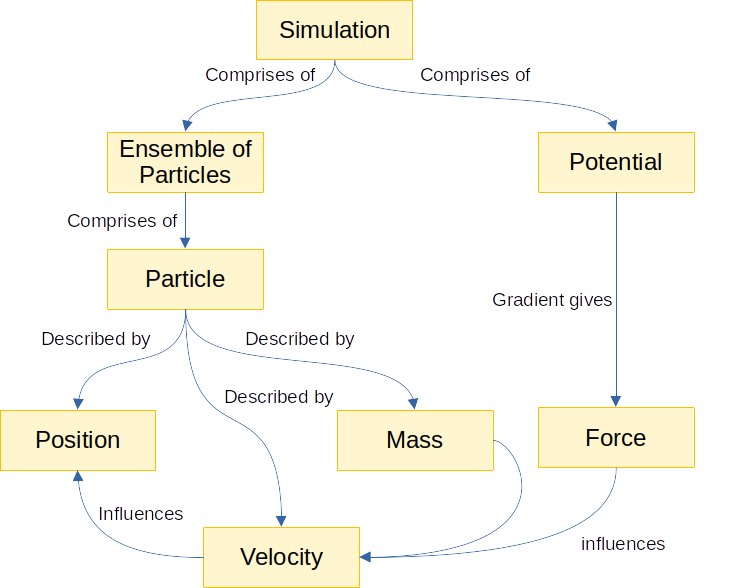
\includegraphics[width=\linewidth]{./gfx/01-structure}
\end{columns}
%
\end{frame}

% =========================================================================== %

\begin{frame}{Classes: Representing Data in Context}
%
\begin{itemize}
\item Remember: \inPy{class}es are data collections plus predefined interactions with the grouped data
\item Essentially: fancy \inPy{dict}s
\item Allows to separate (abstract away) \emph{intent} from \emph{implementation}
	\begin{itemize}
	\item Intent: Method names, \zB \texttt{Potential.get\_force(coordinates)}
	\item Implementation: How is the potential stored in the first place? What data types do I use? Runtime concerns; Failsafes; ...
	\end{itemize}
\item Write \emph{interfaces} first, then go about implementing them
	\begin{itemize}
	\item Interface: Just the method names without any code behind
	\item \inPy{def get_force(coordinates) : pass}
	\item One class for each \emph{sufficiently complex concept} your system features
	\item \emph{Sufficiently complex concept}: Up to debate and personal taste
	\item Rule of thumb: anything which I can ask more questions than \emph{what are your atoms}?
	\end{itemize}
\end{itemize}
%
\end{frame}

% =========================================================================== %

\begin{frame}{Wrapper Classes}
%
Example \inPy{class Particle}:
\begin{itemize}
\item Essentially: group of 5 real numbers (2D case)
	\begin{itemize}
	\item x- and y-position
	\item x- and y-velocity
	\item mass
	\item[\Thus] can (and should) be grouped in one numpy-array
	\end{itemize}
\item But: Readability! Compare ...
	\begin{itemize}
	\item \texttt{particle[0:2]}
	\item \texttt{particle.get\_position()}
	\item \texttt{particle["position"]}
	\end{itemize}
\item And: Custom operations! Compare
	\begin{itemize}
	\item \texttt{particle[0:4] += velocity\_and\_acceleration * dt}
	\item \texttt{particle += velocity\_and\_acceleration * dt}
	\end{itemize}
\item[\Thus] Code should only be concerned with only intent as far as possible!
\end{itemize}
%
\end{frame}

% =========================================================================== %

\begin{frame}{Generic Code vs. Specialized Code}
%
\begin{itemize}
\item Example: number of dimensions
\item Degrees of freedom propagate through your system
	\begin{itemize}
	\item[\Thus] More mental load, more that can break
	\item Often unforseen side effects
		\begin{itemize}
		\item E.\;g.: Increases complexity of computing force field
		\end{itemize}
	\end{itemize}
\item Potentially increases complexity in use
	\begin{itemize}
	\item Need to specify the special case each time used. 
	\item Can sometimes be deduced or taken from default values
	\end{itemize}
\item Advantage in reusability
	\begin{itemize}
	\item Need for generic code may be known from the overall scope of the project
	\item May come unforseen. More often on function/method level than on class level
	\end{itemize}
\item[\Thus] Generalize only if necessary or \emph{very easy}
	\begin{itemize}
	\item Rewriting a \emph{correctly working} piece of code is often difficult enough
	\item Failsafe/easy to use code is worth more than generic code
	\end{itemize}
\end{itemize}
%
\end{frame}

% =========================================================================== %

\begin{frame}{Classes: Order of Implementation}
%
\begin{itemize}
\item (Begin with the interface, maybe only on paper)
\item Write the \inPy{__init__} first
	\begin{itemize}
	\item Which attributes do describe your object?
	\item Which data type and grouping is best suited for this task?
	\item Parameters to the constructor. Again, need not mirror the inner structure.
	\item Example: \texttt{Particle(position, velocity, mass)} (3 parameters). Internally represented by one member (\texttt{data}), which stores five numbers
	\item Thik about default parameters and validity checks
		\begin{itemize}
		\item What if a user accidentally provides a string for either of them?\\
			Usually, just \inPy{raise} an Exception \emph{with meaningful text}
		\item Do I always need to provide all five numbers? Maybe allow \emph{null-initialization}
		\end{itemize}
	\end{itemize}
\item Then: \inPy{__str__}
	\begin{itemize}
	\item Greatly facilitates debugging when you only \inPy{print(particle)} to see\\
		\texttt{Particle at [4.20, 3.14], velocity = [0.00, 0.00], mass = 1.00}
	\end{itemize}
\end{itemize}
%
\end{frame}

% =========================================================================== %

\begin{frame}{Class Methods: Patterns}
%
\begin{itemize}
\item Getters and Setters
	\begin{itemize}
	\item Pattern: attribute \texttt{X} has associated methods \texttt{get\_X(self)} and \texttt{set\_X(self, new\_value)}
	\item Read-only attributes: no setter
	\item Implement, even if trivial
		\begin{itemize}
		\item Trivial getter: \inPy{return self.X}; trivial setter: \inPy{self.X = new_value}
		\item[\Thus] Uniform access for all attributes via getter/setter; later edits affect \emph{all} access points
		\end{itemize}
	\end{itemize}
\item Private attributes and methods begin with underscore
	\begin{itemize}
	\item Many OO languages: private and public members: Acessible only from within class code or from everywhere
	\item[\Thus] Prevent coder from accidentally creating an invalid state
	\item Python: no such concept. (Poor) substitute: naming convention
	\item Message to coder: this is for internal use only. Touch at your own risk
	\item Some IDEs recognize this
	\end{itemize}
\end{itemize}
%
\end{frame}

% =========================================================================== %\\

\begin{frame}{Class Methods: Patterns}
%
\begin{itemize}
\item Grouping subtasks in (pseudo-) private methods
	\begin{itemize}
	\item In particular in constructors
	\item Very useful for reoccuring tasks
	\item Example: \inPy{self.attribute = self._check_if_in_range(inputs)}
	\item Improves code readability, again by separating intent from implementation
	\end{itemize}
\item Method names are verbs, class names are nouns
	\begin{itemize}
	\item Classes model concepts from the physical world \Thus nouns
	\item Methods model what we can do with them \Thus verbs
	\end{itemize}
\item Similar names do similar things (and vice versa!)
	\begin{itemize}
	\item Methods named \texttt{get\_something} should only compute/fetch and return \texttt{something}, without having side effects (changing memory state, producing on-screen output, ...)
	\item If one class has a method \texttt{draw\_something} to create a plot, then another class should not implement a method \texttt{plot\_something}
	\end{itemize}
\end{itemize}
%
\end{frame}

% =========================================================================== %

\begin{frame}{Classes: Order of Implementation}
%
\begin{itemize}
\item Classes themselves: bottom up
\item I.\;e. the "atomic" classes (the elements of composed systems first
\item If mutual interdependence (A affects B, and B affects A; neither is \enquote{element of} the other):
	\begin{itemize}
	\item Avoid if possible, \zB via return values
	\item Start with whichever is easier on your head
	\item Usually the one with fewer active side interactions
	\end{itemize}
\item Building Software bottom up allows to parallelly test the code
	\begin{itemize}
	\item Unittests: Separate program that instantiate your class and use all the methods
	\item Pass if expected results produced
	\item Python offers a number of unittest systems \Thus another evening
	\end{itemize}
\end{itemize}
%
\end{frame}

% =========================================================================== %

\begin{frame}{Classes, Modules and Packages}
%
\begin{itemize}
\item Module: One Python code file
\item Package: A set of modules
	\begin{itemize}
	\item Anything you can load with \inPy{import}
	\item A single module is the smallest form of package conceivable in Python
	\item May have inner structure, on-load-actions, ... (see later)
	\item[\Thus] A way to structure your code
	\end{itemize}
\item Recommendation: One module per class
	\begin{itemize}
	\item Easier to first find the right file out of 20 and then the right method out of 500 lines instead of the right method directly out of 5000 lines of code
	\end{itemize}
\item Additional modules for constants and non-class functions
\item Package mechanism only if you write libraries or have several distinct aspects in your work
	\begin{itemize}
	\item E.\;g.: physics package and visualization package
	\end{itemize}
\end{itemize}
%
\end{frame}

% =========================================================================== %

\begin{frame}{Using Modules}
%
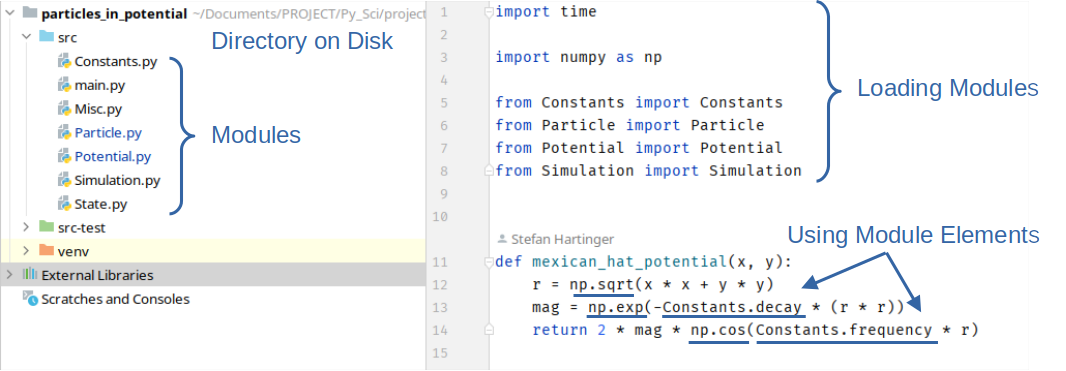
\includegraphics[width=\linewidth]{./gfx/01-modules}
%
\begin{itemize}
\item Simply store your \texttt{.py} files in one directory (here: \texttt{src}) ...
\item ... and load them with \inPy{import} or \inPy{from ... import ...}
\end{itemize}
%
\end{frame}

% =========================================================================== %

\begin{frame}{Using Packages}
%
\begin{itemize}
\item Create an own directory for each package
\item In each package directory, create the file \texttt{\_\_init\_\_.py}
	\begin{itemize}
	\item The directory name is now the package name
	\item The file \texttt{\_\_init\_\_.py} contains setup-code that is executed when running \inPy{import package}
	\item Usually, this is just a number of \inPy{import} commands
	\item Sub-directories within the package directory are denoted with a dot
	\item \inPy{import .Plots.Field}
	\item The first dot means \enquote{relative to the directory of the importing file}
	\end{itemize}
\item You can now \inPy{import package}!
	\begin{itemize}
	\item The objects inside the package are now visible as \texttt{package.object}
	\end{itemize}
\item Side effect
	\begin{itemize}
	\item Python will automatically generate subdirectory \texttt{\_\_pycache\_\_} with \texttt{.pyc} files
	\item Bytecode, essentially machine language version of our code
	\end{itemize}
\end{itemize}
%
\end{frame}

% =========================================================================== %

\begin{frame}{Using Packages}
%
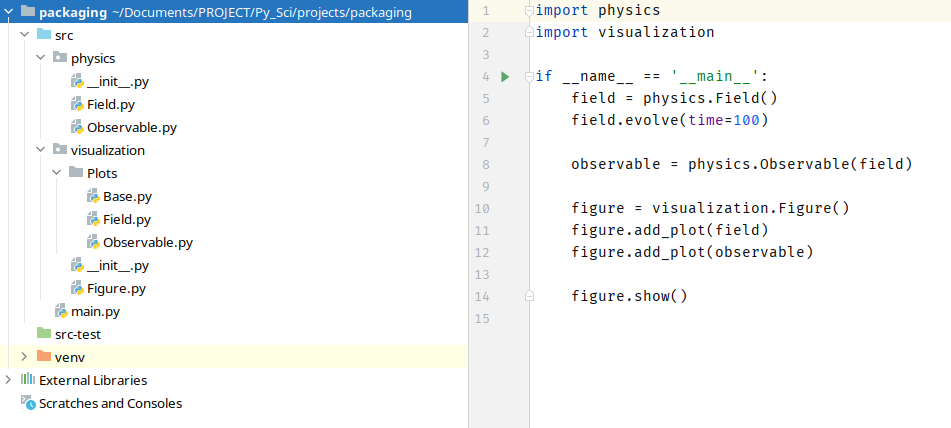
\includegraphics[width=\linewidth]{./gfx/01-packages}
%
\begin{itemize}
\item Simply store your \texttt{.py} files in one directory (here: \texttt{src}) ...
\item ... and load them with \inPy{import} or \inPy{from ... import ...}
\end{itemize}
%
\end{frame}

% =========================================================================== %

\begin{frame}[fragile]{Using Packages}
%
\begin{tcbraster}[raster columns=2,
                  raster equal height,
                  nobeforeafter,
                  raster column skip=0.5cm]
%
\begin{codebox}[\texttt{physics/\_\_init\_\_.py}]
\begin{minted}[fontsize=\scriptsize]{python3}
from .Field import Field
from .Observable import Observable
\end{minted}
\end{codebox}
%
\begin{codebox}[\texttt{visualization/\_\_init\_\_.py}]
\begin{minted}[fontsize=\scriptsize]{python3}
from .Figure import Figure
from .Plots.Observable import *
from .Plots.Field import *
\end{minted}
\end{codebox}
%
\end{tcbraster}
%
\begin{itemize}
\item Note: \texttt{Base.py} is not imported directly by visualization, but indirectly via \texttt{Plots.Observable} and \texttt{Plots.Field}
\item The effect (in \texttt{main.py}) is the same. The \texttt{Base} routines are visible, either way.
\item Note: the code on GRIPS does precisely nothing -- only to illustrate the package mechanism
\end{itemize}
%
\end{frame}

% =========================================================================== %

\begin{frame}[fragile]{Public Interfaces}
%
\begin{defbox}[\texttt{Particle.py} -- Public Interface]
\begin{itemize}
\item \inPy{__init__(self, position=None, velocity=None, mass=None)}
\item \inPy{get_mass(self)} and \inPy{set_mass(self, mass)}
\item \inPy{get_position(self)} and \inPy{set_position(self, mass)}
\item \inPy{get_velocity(self)} and \inPy{set_velocity(self, mass)}
\item \inPy{__getitem__(self, key)} -- forwards to \texttt{get\_X} if \texttt{key} is a string, or accesses underlying numpy array if \inPy{int} or \inPy{slice}
\item \inPy{__setitem__(self, key, value)} -- analogous
\item \inPy{__add__(self, rhs)} (computes \texttt{particle + vector}) and \inPy{__iadd__(self, rhs)} (computes \texttt{particle += vector})
\item \inPy{__str__(self)}
\end{itemize}
\end{defbox}
%
\end{frame}

% =========================================================================== %

\begin{frame}[fragile]
%
\begin{defbox}[\texttt{Misc.py} -- Interface]
\begin{itemize}
\item \inPy{central_difference_quotient(f, x, epsilon)} -- derivative of \texttt{f} in \texttt{x}
\item \inPy{bind_all_parameters_but_ith(f, i, coordinates)} -- transform $f(x_1, ... x_n) \to \tilde{f}(x) = f(x_1, ... x_n) |_{x_i = x}$
\end{itemize}
\end{defbox}
%
\begin{defbox}[\texttt{Constants.py} -- Interface]
\begin{itemize}
\item \texttt{decay} -- form parameter of a decaying oscillation potential used in my example
\item \texttt{frequency} -- form parameter of a decaying oscillation potential
\end{itemize}
\end{defbox}
%
\begin{hintbox}[Partial evaluation of functions]
\small
Python actually has a built-in way of achieving the effect of \texttt{bind\_all\_parameters\_but\_ith}: The module \emph{functools} provides the class \texttt{partial}.\\
See \url{https://docs.python.org/3/library/functools.html}
\end{hintbox}
%
\end{frame}

% =========================================================================== %

\begin{frame}[fragile]
%
\begin{defbox}[\texttt{Potential.py} -- Interface]
\begin{itemize}
\item \inPy{__init__(self, position=None, velocity=None, mass=None)}
\item \inPy{precompute(self, *args)} -- creates a discretized grid to accelerate actual simulation
	\begin{itemize}
	\item Calls \texttt{Misc.bind\_all\_parameters\_but\_ith} and \texttt{Misc.central\_difference\_quotient} for forces
	\end{itemize}
\item \inPy{clear_precomputed(self)} -- restores continuous computation state
\item \inPy{get_nearest_indices(self, coordinates)} -- in discrete mode, find nearest \enquote{pixel} to a given coordinate
\item \inPy{get_expression_potential(self)} and \inPy{get_field_potential(self)} -- return potential as callable lambda and as precomputed array
\item \inPy{get_potential_at(self, coordinates)} and \inPy{get_potential_near(self, coordinates)} -- potential at a given coordinate (continuous/discrete version)
\end{itemize}
\end{defbox}
%
\end{frame}

% =========================================================================== %

\begin{frame}[fragile]
%
\begin{defbox}[\texttt{State.py} -- Interface]
\emph{\small A State is a snapshot of the system: essentially a list of all particles at a given time}
\begin{itemize}
\item \inPy{__init__(self, potential: Potential, particles: list = None)}
\item \inPy{add_particle(self, particle: Particle)}
\item \inPy{evolve(self, dt: float)} -- moves all particles as they would within a time interval \texttt{dt}
	\begin{itemize}
	\item Calls \texttt{Potential.get\_force\_at} or \texttt{Potential.get\_force\_near}
	\item Calls \texttt{Particle.get\_position} and \texttt{Particle.get\_velocity} 
	\item Calls \texttt{Particle.\_\_add\_\_}
	\end{itemize}
\item \inPy{copy(self)} -- creates a copy of the current state
\item \inPy{get_compact_table(self)}  -- converts the current state into a numpy table
\item \inPy{get_compact_table_size(self)}  -- returns the dimensions of the numpy table that \texttt{get\_compact\_table} would return
\end{itemize}
\end{defbox}
%
\end{frame}

% =========================================================================== %

\begin{frame}[fragile]
%
\begin{defbox}[\texttt{Simulation.py} -- Interface]
\begin{itemize}
\item \inPy{__init__(self, potential, partcls=None, t_max=None, dt=None)}
\item \inPy{get_t_max(self)} and \inPy{set_t_max(self)}
\item \inPy{get_dt(self)} and \inPy{set_dt(self)}
\item \inPy{add_particle(self, new_particle)}
\item \inPy{reset(self)}
\item \inPy{advance(self)} adds one timestep to the recorded history
\item \inPy{autorun(self)} adds timesteps until \texttt{t\_max} is reached
\item \inPy{get_compact_table(self)}
\item \inPy{show_plot(self)}
\item \inPy{draw_trajectory_on(self, tab, ax)} and \inPy{draw_speed_on(self, tab, ax)}
\end{itemize}
\end{defbox}
%
\end{frame}

% =========================================================================== %

\begin{frame}[fragile]
%
\begin{codebox}[main.py]
\begin{minted}[linenos, fontsize=\scriptsize]{python3}
# (... some imports ...)

potential = Potential(decaying_oscillation_potential)

sim = Simulation(potential)
sim.set_dt(0.005)
sim.set_t_max(10.0)

sim.add_particle(Particle(position=(+0.90, +0.10),
                          velocity=(-0.10, +0.10),
                          mass=1)
)
sim.add_particle(Particle(position=(-0.90, +0.10),
                          velocity=(-0.10, +0.10),
                          mass=1)
)

sim.autorun()
sim.show_plot()
\end{minted}
\end{codebox}
%
\end{frame}

% =========================================================================== %

\begin{frame}
%
\vspace{-4pt}
\begin{center}
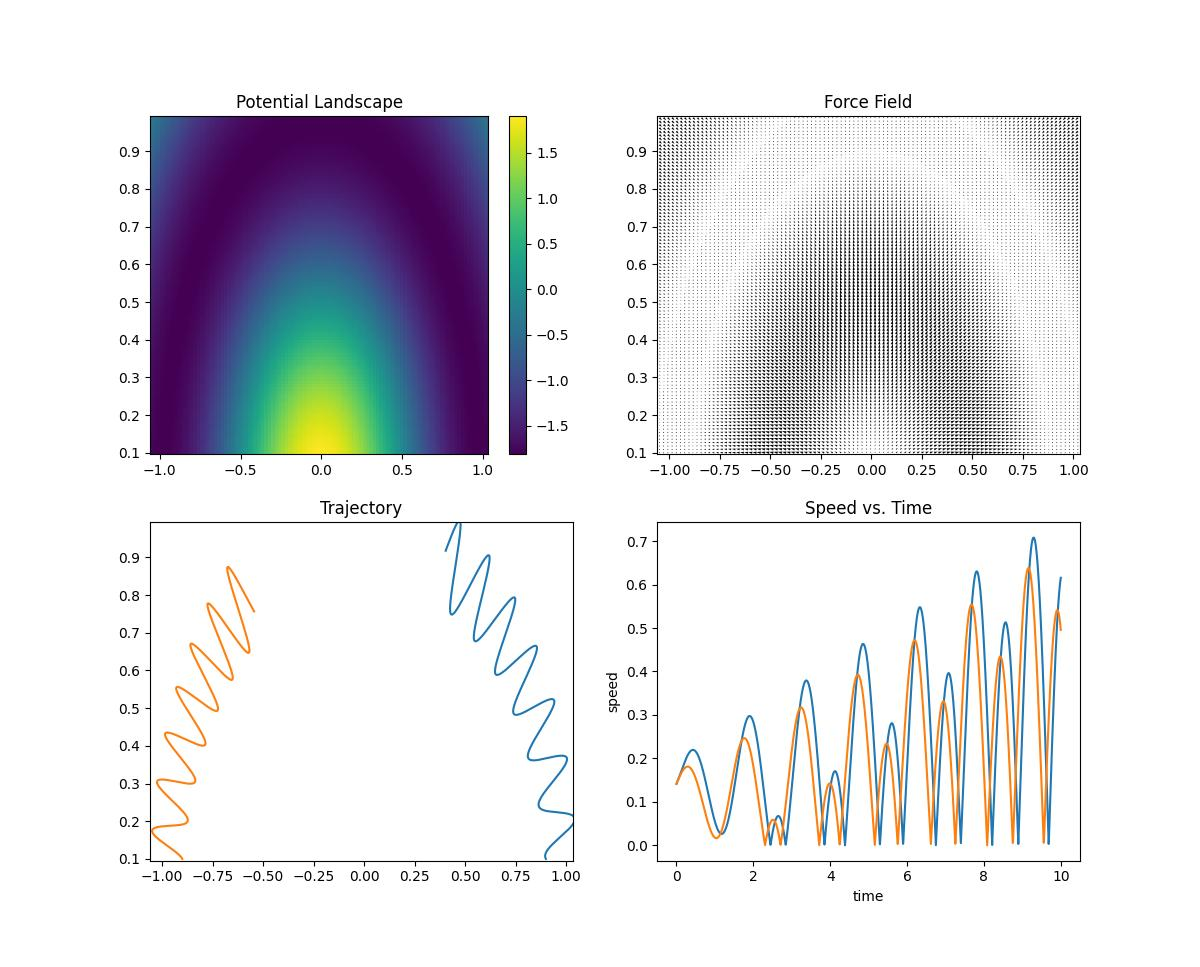
\includegraphics[width=.78\linewidth]{./gfx/01-result}
\end{center}
%
\end{frame}